\cleardoublepage
\newrefsection
\chapter{文献综述}

\section{背景介绍}
情绪是人对客观事物的态度体验及相应的行为反应,它不仅是影响个体个性特征和心理及生理健康的关键因素,
还在人类学习、记忆、注意力和决策等机制的发展中起到重要作用。因此近年来,如何对情绪进行客观评估逐渐成为研究热点,
在医疗健康、人工智能、远程教育等多个领域均有广泛的应用前景。

在医疗健康领域,通过健康监控,我们可以创建情绪相关的个人健康档案,帮助识别压力、焦虑、抑郁或慢性疾病的部分诱因,
并辅助后续的情绪干预治疗;在人工智能领域,如自动驾驶辅助报警系统,我们可以在汽车原有组件(如方向盘)中集成生理信号监测模块,
通过非侵入式技术无创地监测用户的生理状态,在用户感到困倦、不舒服甚至失去意识无法驾驶时适时发出警告,
并在必要时减速或停车,以获得更安全的驾驶体验\cite{Placido2012};在远程教育领域,我们可以通过监测个体在不同教学实践中的生理参数变化,
对学习材料和教学安排进行适当个性化的调整,以提升教学效率和人机交互效果。

心理学研究表明,情绪不仅有个体的主观体验和外部行为表现,同时还伴随着复杂的生理变化和神经机制。
情绪通常可由面部表情、姿态表情和语调表情等外显特征进行识别,然而这类特征很大程度上依赖于个体的社会环境、
文化背景和个性,容易被人为掩饰或伪装﹐难以排除主观因素的影响,有时甚至可能获知相反的情绪状态。
而伴随情绪的生理反应则不存在这些限制(如心率加快、出汗、瞳孔放大等),它由神经和内分泌系统支配,具有自发性,
不易受到主体控制而能够反应出更加真实的主体情感体验。
在生理信号中,心电、脉搏、呼吸等外周自主神经反应的测量和信号采集较脑电等中枢神经反应更加简便和易于分析,
对于实验环境和设备的要求以及对于被试的干扰都更低,也更符合未来实际应用的需求。

论文旨在梳理基于外周生理信号的情绪识别研究现状,从情绪识别的基本理论、
实验范式和分析方法等方面系统回顾了领域内的典型成果和部分最新研究,
归纳总结了近年来的研究进展和目前存在的研究难点以及未来更具潜力的研究方向。


\section{国内外研究现状}

\subsection{研究方向及进展}
 
\subsubsection{理论背景}

1.情绪模型

情绪识别面临的首要问题是如何进行情绪分类,即建立情绪模型。采用通用统一的情绪模型有利于提升不同研究间的可比性和推广性,目前心理学界主要有两种主流的情绪模型,即离散情绪模型和维度情绪模型。

% \begin{enumerate}[\qquad(1)]
%     \item 离散情绪模型
% \end{enumerate}
    
% \hangafter 0
% \hangindent 1.6em
(1)离散情绪模型:即情绪分类取向,源于Darwin的进化论思想\cite{Darwin2015},其研究者认为情绪主要由几种相对独立的基本情绪以及由基本情绪结合形成的多种复合情绪所构成。
Tomkins\cite{Tomkins1970}较早提出了存在八种原始情绪,即惊喜、兴趣、喜悦、愤怒、恐惧、厌恶、耻辱和痛苦。
% 兴趣—兴奋、享受—快乐、惊奇—吃惊、苦恼—痛苦、厌恶—轻蔑、愤怒—狂怒、羞耻—耻辱、惧怕—恐惧。
Ekman\cite{Ekman1971,Ekman1992}则将情绪描述为离散的、可测量的和与生理学相关的,
% 具有生理意义和交流功能。基于以上理解,他
存在快乐、悲伤、愤怒、恐惧、厌恶和惊讶六种基本情绪,该基本情绪分类学说也成为目前影响力最大的情绪分类方法之一。
Izard\cite{Izard1991}基于情绪分化理论将基本情绪分为十种,包括快乐、悲伤、愤怒、恐惧、厌恶、惊讶、兴趣、害羞、自罪感和蔑视。
Plutchik\cite{Plutchik2001}则提出了一种情感轮模型的情绪分类方法(如\autoref{fig:Plutchik_wheel}所示),将基本情绪分为快乐与悲伤、恐惧与愤怒、接受与厌恶、惊讶与期待四组对立情绪,并在此基础上垂直扩展出表征情绪强度的第三维。
虽然这些基本情绪的分类不尽相同,但本质都在于用独立具体的词汇去描述情绪,而没有对情绪进行定量分析。
同时,后续一项关于自主神经活动与情绪关系的研究也模型提出了挑战,其研究结果表明,不同的基本情绪可能产生相似的神经生理反应,而不同的神经生理活动也可能出现在相同的基本情绪中\cite{Cacioppo2000}。
因此,离散情绪模型对于情绪及其强度变化,尤其是复杂情绪,缺乏进一步的分析能力,不利于研究实际环境中人类所能表达出的丰富情绪词汇。

% \begin{enumerate}[\qquad(2)]
%     \item 维度情绪模型
% \end{enumerate}

% \hangafter 0
% \hangindent 1.6em
(2)维度情绪模型:即情绪维度取向,认为情绪是高度相关的连续体,无法区分为独立的基本情绪,并且同类情绪在其基本维度上都高度相关,但有关基本维度的数量和类型还存在一定争议。
Wundt\cite{Wundt1896}最早提出情绪的三维学说,认为情绪过程由三对情绪元素组成,即愉快-不愉快、兴奋-沉静、紧张-松弛,
并且每对元素都有两极之间的程度变化。Schlosberg\cite{Schlosberg1954}根据面部表情的研究,在Wundt三维学说的基础上提出愉快-不愉快、注意-拒绝、激活水平的三维理论。
Mehrabian和Russell\cite{Mehrabian1974}提出了情绪状态的三维度模型,即愉悦度(或称效价,论文中统一使用效价进行表述)-唤醒度-支配度(PAD),
其中效价的范围从消极到积极,表示情绪从不愉快到愉快;唤醒度的范围从被动到主动,表示情绪的激烈程度,
支配度的范围从受控到主控,表征个体在某种情绪中的控制能力。不同的情绪都可以根据这三个维度的不同特性在情绪空间中被区分开来(如\autoref{fig:PAD}所示)。
后来,Russell\cite{Russell1980}认为支配度更多地与认知活动有关,效价和唤醒度已经能够解决绝大部分情绪变异,由此提出环形模型(又称效价-唤醒模型,如\autoref{fig:Russell}所示)。
维度情绪模型通过连续维度的表征方式,抽离出不同情绪之间的共性并在此基础上构建空间体系,以便对情绪进行定量分析,摆脱了离散情绪模型在复杂情绪表征上的局限,也更适用于研究及实际应用。

\setlength{\belowcaptionskip}{-0.3cm}
\begin{figure}[htbp]
    \centering
    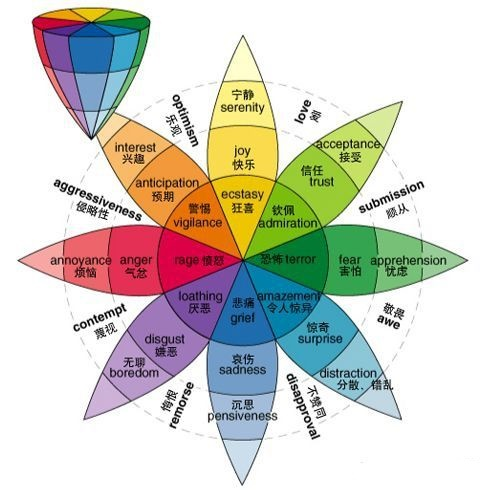
\includegraphics[width=.48\linewidth]{Plutchik wheel.jpg}
    \caption[Plutchik情绪轮模型示意图]{ Plutchik情绪轮模型示意图}{\label{fig:Plutchik_wheel}}
\end{figure}

\setlength{\belowcaptionskip}{-0.3cm}
\begin{figure}[htbp]
    \hspace {0.1cm}
	\centering
	\begin{minipage}[l]{0.44\textwidth}
		\hspace {-1cm}
        \centering
		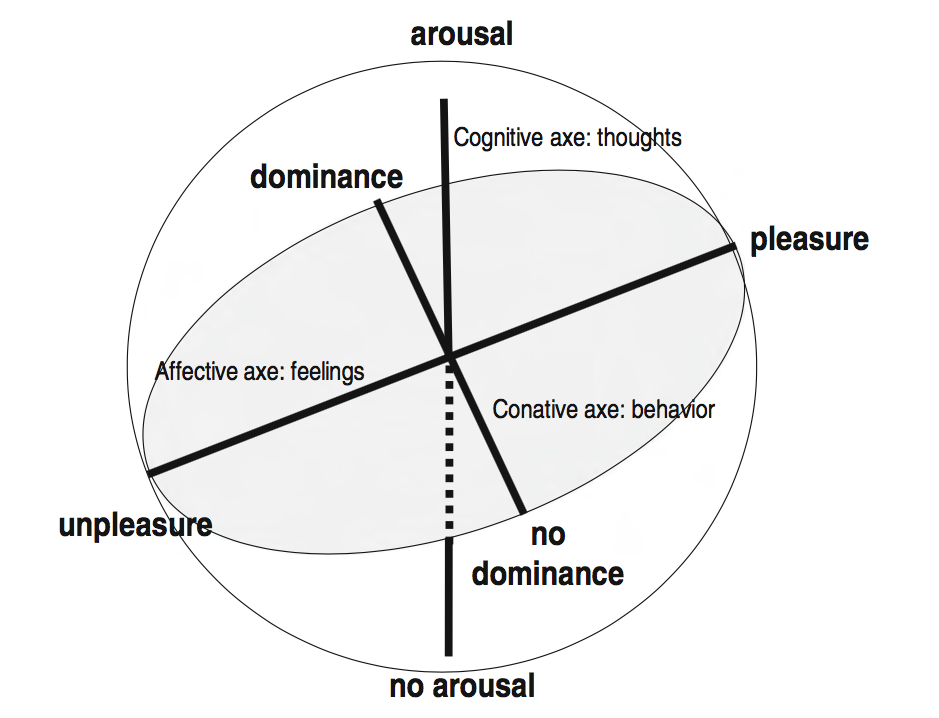
\includegraphics[width=\textwidth]{PAD.png}
		\caption{PAD模型示意图}
		\label{fig:PAD}
	\end{minipage} 
	\begin{minipage}[c]{0.53\textwidth}
		\hspace {-2cm}
        \centering
		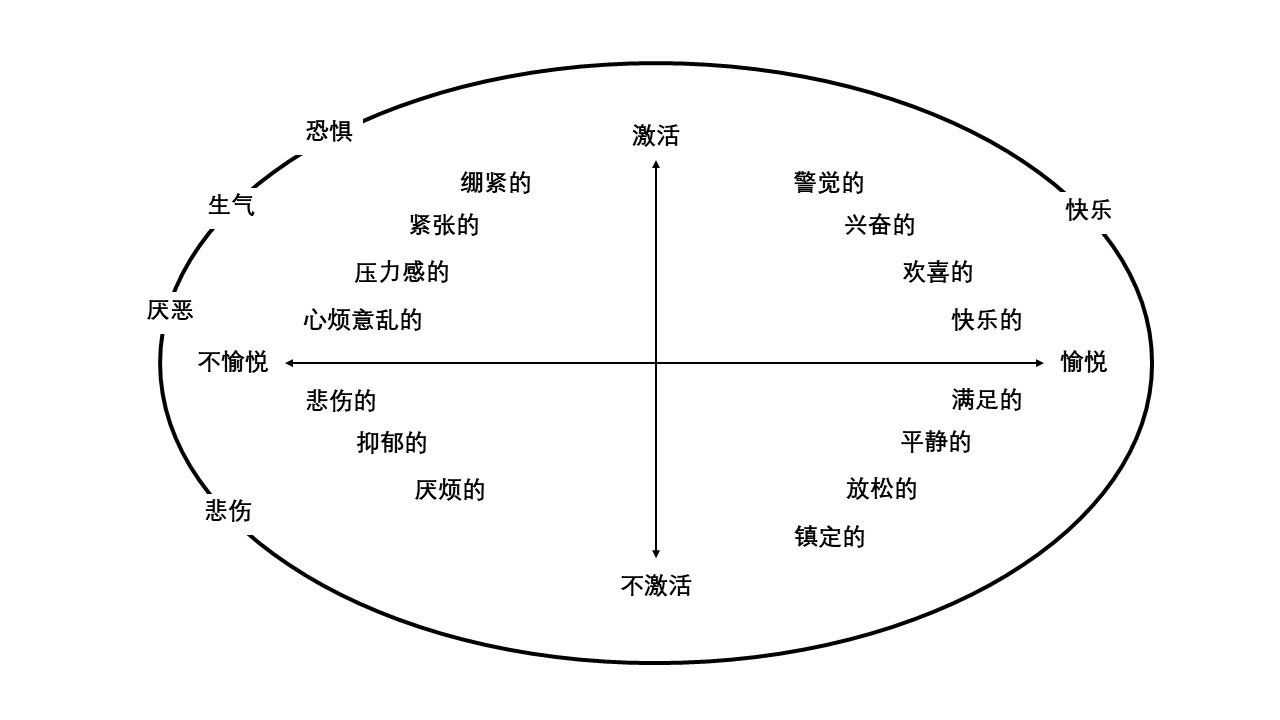
\includegraphics[width=1.2\textwidth]{Russell.jpg}
		\hspace {-2cm}
        \setlength{\abovecaptionskip}{-0.01cm}
        \caption{Russell环形模型示意图}
		\label{fig:Russell}
	\end{minipage}
\end{figure}

2.情绪自主神经系统反应的相关理论

如前文所述,任何情绪体验都伴随着一系列的生理唤醒,包括外周自主神经系统的反应、大脑脑区的活动变化以及体内一些神经化学物质的改变。
论文所聚焦的外周生理信号,它与情绪活动之间的密切联系一直在情绪生理机制的研究中占据重要地位。

早期美国科学心理学之父William James\cite{James1884}在1884年提出,情绪是由某些刺激引起的外周生理变化的结果而非生理变化的前提,情绪体验是个体对外周生理反应的知觉反馈,
这种反应主要是指外周神经系统支配下的内脏和腺体的运动,不同的情绪伴随独特的生理变化(如心率、血压等)模式和骨骼肌的运动变化。
继James之后,丹麦心理学家Lange也提出类似的观点,认为情绪是内脏活动的结果,强调情绪与血管变化的关系。
Malatesta等\cite{Malatesta1987}将情绪定义为“神经过程的特殊组合,引导特定的表达和相应特定的感觉”。据此,一些研究者试图通过多种实验手段找到人类基本情绪所对应的外周生理反应模式,
也确实发现人类所体验到的不同情绪在皮肤、心率、血压、指温、心率变异性等生理指标上存在一定的差异\cite{Kreibig2010},为后续研究建立基础。

\subsubsection{实验范式}

1.情绪诱发方式

在实验室中考察情绪体验的生理机制,需要可靠有效的情绪诱发和控制方法。
情绪诱发方法是指“在非自然和严格控制的条件下唤起个体临时性情绪状态的策略”\cite{Banos2006}。
目前,有关基本情绪状态下的自主神经反应的研究主要有以下几种典型的情绪诱发方式:

% \begin{enumerate}[\qquad(1)]
%     \item 电影片段情绪诱发
% \end{enumerate}
    
% \hangafter 0
% \hangindent 1.6em
(1)电影片段情绪诱发方法:通过观看电影或其他视频片段来诱发被试特定的情绪状态,要求被试在观看过程中对产生的情绪不加抑制,使其自然流露。
Baldaro等\cite{Baldaro2002}通过一些出现肢体严重损伤或受伤流血画面的影片(暴力威胁和外科手术等)来诱发被试情绪,发现被试的皮肤电导水平升高而心率下降。
Gomez等\cite{Gomez2005}采用影片诱发范式,发现高唤醒情绪使得被试的呼气时间较低唤醒情绪更短,而吸气时间占呼吸总时间比例则更高,平均呼气流量和每分钟通气量也更大。
目前,每分钟通气量随着情绪唤醒度的上升而增大的结论,已经得到了较为一致的证明,被认为是呼吸系统中最可靠的用于衡量情绪唤醒度的指标。
徐景波等\cite{XuJingbo1995}选用《猫和老鼠》和《黑太阳七三一》两段电影片段分别诱发正性和负性情绪,发现正性情绪下被试心率变化不显著,指端脉搏容积显著下降,而负性情绪下被试心率显著增加,指端脉搏容积显著下降。
李建平等\cite{LiJianping2006}选用《我的兄弟姐妹》、《午夜凶铃》等六段电影片段诱发92名被试五种基本情绪,发现悲伤、愤怒、恐惧及中性片段导致收缩压升高,厌恶、愤怒、恐惧、快乐和中性片段导致呼吸频率加快,悲伤、恐惧和中性片段导致HRV高频功率降低。
贾静等\cite{JiaJing2008}选用《活着》、《憨豆先生》和《企鹅日记》三段影片分别诱发悲伤、快乐和中性情绪,发现悲伤和快乐情绪都会导致被试呼吸频率降低,而悲伤情绪还能引起皮肤电电位的增高。电影片段诱发情绪的方法已经在大量研究中被应用和验证,在使用上更具灵活性和针对性。

% \begin{enumerate}[\qquad(2)]
%     \item 文字/图片情绪诱发
% \end{enumerate}
    
% \hangafter 0
% \hangindent 1.6em
(2)文字/图片情绪诱发方法:通过连续观看具有强烈情绪色彩的图片或文字来诱发被试特定的情绪状态,并测量诱发情绪的持续时间。
Gomez等\cite{Gomez2004}采用不同正负效价和唤醒度的情绪图片来诱发情绪,发现随着图片效价的增加,被试吸气时间延长,平均吸气流量减少,胸式呼吸增加;随着图片唤醒度的增加,被试吸气时间和总呼吸时间缩短,平均吸气流量、每分钟通气量、胸式呼吸和皮肤电活动增加。
% Carson Smith采用快速呈现情绪图片的方法,发现被试皮肤导电性在呈现负性情绪图片时显著上升,而在呈现正性或中性图片时显著下降。
Bradley等\cite{Bradley2008}的研究发现,采用高情绪唤醒度(不论正性或负性)图片诱发情绪时,被试瞳孔直径变化和皮肤电导水平变化显著。
后续Laukka等\cite{Laukka2013}进一步发现,瞳孔在负性、中性、正性图片中的扩张程度依次减小且差异显著。
目前常用的情绪图片诱发材料是由美国国立精神卫生研究所建立的标准化国际情绪图片库(IAPS)和英语情感词/短文系统(ANEW/ANET)。
同时,白露等\cite{BaiLu2005}建立了本土化的中国情绪图片/词库 (CAPS),在中国群体情绪诱发的针对性研究上进行了探索。

% \begin{enumerate}[\qquad(3)]
%     \item 录音/音乐情绪诱发
% \end{enumerate}
    
% \hangafter 0
% \hangindent 1.6em
(3)录音/音乐情绪诱发方法:通过听具有强烈情绪色彩的音乐(如鸟叫、婴儿哭泣、炸弹爆炸等)来诱发被试特定的情绪状态。
Partala等\cite{Partala2003}采用10段高唤醒度的负性、正性及中性声音,发现被试瞳孔直径在正负性声音条件下显著大于中性条件,且正负性刺激分别使得女性、男性出现最大瞳孔变化。
Kallinen\cite{Kallinen2004}让被试分别在睁眼和闭眼条件下听四段不同效价和唤醒度的音乐片段,发现被试皮肤电导水平随正负性情绪唤醒水平的增高而增高。
刘贤敏等\cite{LiuXianmin2011}选取两段旋律相间但演奏乐器不同(古筝和埙)的乐曲,诱发出悲伤和愉快两种完全不同的情绪,同时发现愉快情绪下被试的皮肤温度高于悲伤情绪,心率变化则受到情绪和性别的交互影响。
目前NIMH建立的国际情感数码声音系统(IADS)和
刘涛生等\cite{LiuTaosheng2006}建立的本土化的中国情感数码声音系统(CADS)为探讨音乐诱发情绪的自主神经反应提供了标准化的实验刺激材料。

% \begin{enumerate}[\qquad(4)]
%     \item 自传式回忆/想象情绪诱发
% \end{enumerate}

% \hangafter 0
% \hangindent 1.6em
(4)自传式回忆/想象情绪诱发方法:通过让被试想象某种情境来达到情绪内部诱发的目的。
Brewer等\cite{Brewer1980}在1980年提出自传式回忆方法,指导被试通过回忆相应的自传式事件来诱发特定情绪。
Wright和Mischel\cite{Wright1982}在1982年提出想象情绪诱发方法,指导被试通过想象一些悲伤、愉快、中性等情景(可以是想象虚构,也可以是过去真实经历),并身临其境地感受与思考。
Sinha等\cite{Sinha1992}采用该情绪诱发方法发现,愤怒和恐惧情绪会导致被试收缩压升高,同时愤怒情绪还会导致舒张压升高。
Neumann和Waldstein\cite{Neumann2001}的研究发现,回忆个人情绪性事件整体上使得被试血压、心率、总外周阻力显著增强,而心搏指数显著下降,同时收缩压在负性情绪中显著高于正性情绪。
然而,通过自传式回忆或想象诱发情绪的局限在于需要专业人士的指导以及被试有意识的合作,在具体操作以及对情绪诱发持续时间和强度的把握上会存在一定的难度。

% \begin{enumerate}[\qquad(5)]
%     \item 具身情境性情绪诱发
% \end{enumerate}

% \hangafter 0
% \hangindent 1.6em
(5)具身情境性情绪诱发方法:通过模拟和操控一些真实情境来诱发与改变被试的情绪体验,诱发效果出色但操作难度上升。
Egloff等\cite{Egloff2002}通过让被试进行演讲的方式诱发其焦虑情绪,发现被试的指端脉搏容积和呼吸频率下降,心率和血压则显著增加。
Britton等\cite{Britton2006}的研究进一步发现,被试的皮肤电和心率变化在进行有关负性主题的演讲时更为显著。
同时,随着虚拟现实(VR)技术的快速发展,应用VR来诱发情绪的相关研究也不断涌现。

此外还有一些研究中较少使用的情绪诱发方式,如面部操作任务诱发(指导被试做不同基本情绪状态下的面部表情)、气味情绪诱发(让被试有意识或无意识地闻某种气味)以及组合情绪诱发(组合两种或两种以上的情绪诱发方式)等,论文不做详细介绍。

2.情绪评估方法

情绪可以通过外部和内部两种方法进行评估。外部评估,即外部注释者根据被试对外可观察到的行为和生理反应来评价其情绪状态,这种方式依赖于多种因素(如个体性格、环境、文化等),受制于被试对情绪体验的外化能力。
因此,情绪识别的相关研究主要使用内部(自我)评估方法进行情绪评价。

其中,应用最广泛的为自我评估量表(SAM)\cite{Bradley1994},它通过连续的9点视觉量表对情绪反应进行主观评价。
如\autoref{fig:SAM}所示,效价轴模型从微笑到皱眉,表示情绪从愉快到不愉快;唤醒度轴模型从闭眼到睁眼,表示激活度从低到高;支配度轴模型由小变大,表示从被控制/服从到控制/强大。
另一常用量表为正-负性量表(PANAS),由两组情绪量表组成,积极情绪轴反映热情、激活和警觉程度,消极情绪轴则反映痛苦和不愉快程度\cite{AMIGOS2017}。
此外,生态瞬时评估(EMA)技术也逐渐受到关注,该方法要求被试间隔若干小时或在某一事件发生时自我报告其想法、感觉、行为和背景环境,有助于分析个体在日常生活中的情绪变化。

在情绪评估量表之外,研究中通常还使用大五人格模型评估来辅助情绪分析\cite{AMIGOS2017},从外倾性(社交型或矜持型)、宜人性(有同情心或冷静多疑)、责任心(有责任心或随意))、神经质性(紧张或自信)和开放性(好奇或谨慎)五个维度来评估个体人格,并对情绪刺激实验中产生的个体差异进行解释。
\begin{figure}[htbp]
    \centering
    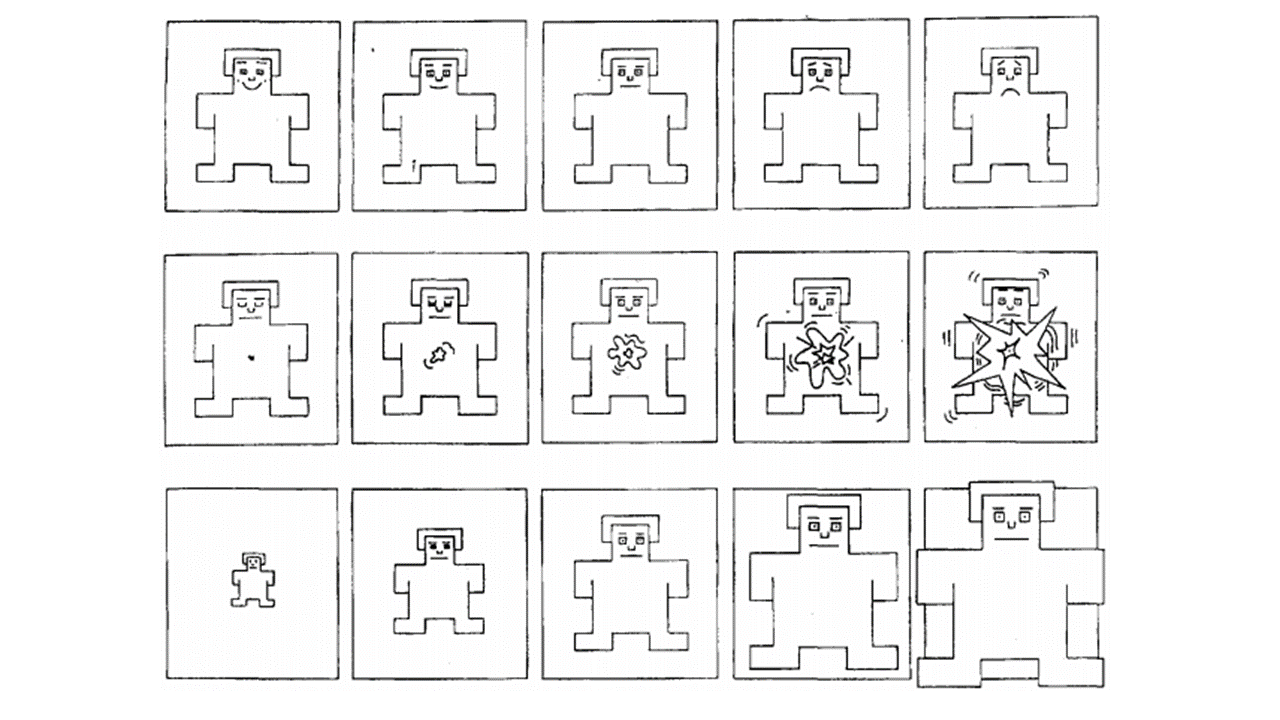
\includegraphics[width=.95\linewidth]{SAM.png}
    \caption[SAM自我评估量表]{SAM自我评估量表:从上到下依次为效价轴、唤醒度轴和支配度轴}{\label{fig:SAM}}
\end{figure}

\subsubsection{分析方法}

情绪刺激实验完成后,研究中主要按照以下步骤对信号进行分析:

1.信号预处理

实验室中诱发的情绪通常难以保持稳定,且生理信号在采集过程中易受到噪声或其他因素的干扰(如环境温度和湿度不稳定、被试生理功能障碍、被试移动、电极断开、静电伪像等),故需进行信号预处理以保留有效数据段。
其主要流程包括同步生理信号,截取情绪诱发效果最佳的数据段,删除有损数据和空值并通过线性插值补充数据,去除噪声、伪迹等干扰。由于生理信号类型和研究目标的不同,研究中具体使用的滤波器类型及其频带参数等特性各不相同,
如Murugappan等\cite{Murugappan2013}使用截止频率为0.002Hz和100Hz的三阶巴特沃斯滤波器以消除ECG信号中噪声和基线漂移的干扰;
Elgandi\cite{Elgendi2012}使用截止频率为1Hz和8Hz的4阶带通滤波器以去除脉搏信号噪声并增强特征;
Wardana\cite{Wardana2017}则使用截止频率为0.15Hz的30阶FIR滤波器以去除呼吸信号噪声并平滑信号。
同时,由于不同被试的生理信号基线之间普遍存在个体差异,部分研究中还对生理信号进行了进一步的归一化处理\cite{Mandryk2007}。

2.模型处理

对信号进行预处理后,研究中主要采用传统的机器学习方法对信号进行特征的提取、选择与融合处理以构建、优化情绪识别模型。

% \begin{enumerate}[\qquad(1)]
%     \item 特征提取
% \end{enumerate}

% \hangafter 0
% \hangindent 1.6em
(1)特征提取:研究中外周生理信号的常用特征如\autoref{tab:signal-feature}所示。除常规的时域和频域特征外,生理信号还具有非常复杂的非线性特征,这些特征与大脑、神经和心脏等部位的活动高度相关,可以反映情绪的调控过程。
相关研究证明\cite{Valenza2012,Khaliliardali2015},使用熵值、关联维数等非线性特征可以获取信号在复杂程度、混乱程度和不确定程度等方面的信息,能有效表征情感活动。
C. Li等\cite{LiCailong2018}使用递归图和递归定量分析的方法从EMG、SKT和RESP中提取非线性特征,分类效果较传统时频和统计特征更好。
Rubin等\cite{Rubin2016}在恐惧状态的识别中将ECG信号的传统时频域特征和非线性特征相结合,显著提升了模型准确度。
因此,非线性特征的发展与提取是目前情绪识别领域的一个研究重点。

% \begin{enumerate}[\qquad(2)]
%     \item 特征选择
% \end{enumerate}

% \hangafter 0
% \hangindent 1.6em

\begin{table}[htbp]
    \centering
    \footnotesize
    \setlength{\abovecaptionskip}{0.1cm}
    \setlength{\belowcaptionskip}{0.2cm}
    \renewcommand\arraystretch{1.5}
    \caption[常用外周生理信号及其模态特征。]{常用外周生理信号及其模态特征\cite{Bota2019}}
    \label{tab:signal-feature}
    \begin{tabular}{@{}lll@{}}
    \toprule
    信号                                                                                  & 模态  & 特征                                                                                                                                                           \\ \midrule
\multirow{4}{*}{\begin{tabular}[c]{@{}l@{}}    \\心电(EEG)/\\ 光电容积脉搏波\\ (PPG)\end{tabular}} 
                                                                                    & 时域  & \begin{tabular}[c]{@{}l@{}}一些基本时间特征(最大/小值、均值、中值、标准差及其比值、差值等),\\ 连续RR间期差异大于20ms(pNN20)或50ms(pNN50)的数量及百分比,\\pNN5O/pNN20比值, RR间期直方图的积分/高度比值、基线宽度等\end{tabular} \\
                                                                                    & 频域  & \begin{tabular}[c]{@{}l@{}}总能量,超低频段(ULF,0-0.003Hz)、极低频段(VLF,0.003-0.03Hz)、\\ 低频段(LF,0.03-0.15Hz)、高频段(HF,0.15-0.4Hz)、归一化低频和高频、\\ LF/HF比值、总光谱功率等\end{tabular}  \\
                                                                                    & 非线性 & 谱熵、小波熵、近似熵、样本熵,关联维数,Lempel-Ziv复杂度                                                                                                                            \\ \midrule
\multirow{2}{*}{\begin{tabular}[c]{@{}l@{}}  皮肤电EDA\end{tabular}}                  & 时域  & \begin{tabular}[c]{@{}l@{}}SCL线性度,SCR信号的时间特征、事件数、事件下面积,\\ SCR幅值的时间特征、上升和50\%/60\%恢复时间\end{tabular}                                                             \\
                                                                                    & 频域  & \begin{tabular}[c]{@{}l@{}}0-2.4Hz频段10谱功率,0-0.2Hz内的皮肤电导慢响应SCSR,\\ 0-0.08Hz内的皮肤电导极慢响应过零率SCVSR等\end{tabular}                                                   \\ \midrule                                    
                                                                                    
\multirow{3}{*}{\begin{tabular}[c]{@{}l@{}}   \\ 呼吸RESP\end{tabular}}              & 时域  & \begin{tabular}[c]{@{}l@{}}呼吸频率/节律,吸气(I)和呼气(E)持续时间及I/E比值、\\ 伸展(一个呼吸周期的峰值和最小振幅的差值)、平均/中位峰峰时间\end{tabular}                                                     \\
                                                                                    & 频域  & \begin{tabular}[c]{@{}l@{}}在0-0.1Hz、0.1-0.2Hz、0.2-0.3Hz和0.3-0.4Hz内的相关频域特征,\\ 0-2.4Hz频段10谱功率\end{tabular}                                                     \\
                                                                                    & 非线性 & 谱熵、小波熵、近似熵、样本熵,关联维数,Lempel-Ziv复杂度           
                                                                                                                                                                                                      \\  \bottomrule
    \end{tabular}
    \end{table}

% \begin{enumerate}[\qquad(3)]
%     \item 特征融合
% \end{enumerate}

(2)特征选择:特征提取完成后,通常会因为其数量过多而导致维度灾难,此时就使用特征选择来降低数据维度,具体方法大致可以分为过滤式、包裹式和嵌入式三类。
过滤式方法首先通过设定准则(常用Fisher Score方法\cite{Boonthong2015}、ReliefF方法\cite{ZhangJianhai2015}等)对特征进行排序和选择,然后再训练模型,特征选择过程与后续模型训练无关,选择的是原特征集的子特征集。这种方法较为简便,但缺陷在于它忽视了被选择的特征子集对于分类器性能的影响。
针对这一问题,包裹式方法通过使用一个分类器对不同特征的质量以及不同特征子集的结果进行评估加以改善,如应用前向选择与后向消除的典型方法。包裹式方法能有效提升模型性能,但缺陷在于必须对所有特征进行穷尽搜索,计算复杂度很高。
针对这一问题,嵌入式方法通过将前两种方法结合的方式加以改善,即先采用过滤式方法降低特征选择空间的大小,再基于这些特征使用包裹式方法以最大限度提升性能。

% \hangafter 0
% \hangindent 1.6em
(3)特征融合:研究表明,使用不同的信号模态可以提升分类性能\cite{DEAP2011}。模态融合主要分为特征融合和分类器融合两类,前者从每种模态中提取特征并标准化处理后,拼接成一个特征向量空间作为机器学习模型的输入;
后者则通过决策层融合,将每种模态提取的特征作为分类器的输入,分类器训练需要并行执行以减少计算时间。特征层融合的实现难度和计算复杂度都相对较低,但它需要同步化不同模态的数据且无法应对低质量数据,
而决策层融合则不需要。同时,决策层融合能够运用权重调整每种模态对结果的贡献\cite{DEAP2011},能够进一步改善分类效果。


3.模式识别

传统的基于模型的机器学习分类方法分为监督、非监督和半监督方法。

监督学习(SL)方法将生理信号特征映射到相应标签以创建模型,常用算法包括朴素贝叶斯(NB),k近邻(K-NN)、支持向量机(SVM)、线性判别分析(LDA)和二次判别分析(QDA)等。
其中,SVM分类器应用最为广泛,其次是K-NN和RF分类器。例如,何成等\cite{HeCheng2017}基于ECG和RESP的SVM数据识别愉悦和悲伤情绪,准确率分别为分别为81.82\%和63.64\%。
Myroniv等\cite{Myroniv2017}基于RT、DT、NB、KNN、SVM和MPNN模型对HR、GSR和SKT信号进行分类,其中KNN模型的平均准确率达到了最高的97.78\%。

非监督学习(UL)方法区别于监督学习方法,训练数据只有特征而没有标签,需要自己进行聚类分析并提取结构,常用算法包括k均值、亲和传播、光谱聚类、层次聚类、高斯混合模型(GMM)等。
例如,Adams等\cite{Adams2014}基于GMM模型对EDA信号在唤醒度维度上进行二分类,得到了74.3\%的准确率。
Birjandtalab等\cite{Birjandtalab2016}基于GMM模型对EDA、HR和${\rm SpO}_{\rm 2}$信号进行分类,针对放松、生理紧张、情绪紧张和认知紧张这4种状态均得到了大于84\%的准确率。

\raggedbottom
半监督学习(SSL)方法则是以上两种方法的结合,同时使用未标记数据和标记数据进行分析,常用算法包括自我训练(ST)和主动学习(AL)等。
例如,X. Jia等\cite{JiaXiaowei2015}对EEG数据使用进行SSL方法,使其模型的分类效果显著提升并优于大部分模型。

4.模型评估

\raggedbottom
模型评估是对模型效果的验证,以检验模型应用于未知数据的分类效果。常用方法是将数据分为训练集(用于训练模型)、验证集(用于调整超参数,部分研究不设置)和测试集(用于获得评估模型性能)。
研究中一般使用k折交叉验证(CV)的方法,将原数据集划分为k个等大子数据集(1个用于测试,其余用于训练),迭代k次后将测试集的分类结果取平均值作为输出以评价模型。
具体的评价参数包括正确率(正确分类样本的百分比)、查准率(真正例在预测的正例中所占的比例)、特异性(预测的真负例所占所有真负例的比例)、F1分数(查准率和查准率的调和平均值)和均方误差(数据集中每个样本均方误差的平均值)五项。

除传统机器学习方法之外,不依赖于特征的深度学习方法(DL)也逐渐应用到情绪识别的研究当中。
杨一龙等\cite{YangYilong2018}使用一种结合CNN和RNN的混合神经网络,通过学习原始EEG数据的组成时空表征来区分情绪状态,最终将情绪识别准确率提高了约32\%,在效价分类和唤醒分类上的平均准确率分别为90.80\%和91.03\%。
陈景霞等\cite{ChenJX2019}提出一种基于CNN模型的使用EEG特征进行情绪分类的模型,并对比了该模型与决策树、支持向量机、线性判别分析、贝叶斯线性判别分析等在DEAP标准情绪数据集上的识别效果,发现深度学习模型在结合时域与频域的特征集上获得了最好的识别效果。利用深度学习进行情绪识别的有效性在大量研究中得到证明,
其识别效果与准确率甚至优于部分传统的机器学习模型,但其缺陷在于解释性很差,不能表征生理信号和情绪之间的对应关系,同时也需要大量的数据和较高的计算成本。

% \subsubsection{典型数据库}

\subsection{存在问题}
综上所述,目前已经有许多基于生理信号进行情绪识别的研究。随着研究的深入,诱发的情绪种类逐渐复杂,使用的生理信号变得多样化,提取的特征参数更为有效,识别模型的性能也逐步提升。在完善情绪诱发方案,构建标准情绪数据库,
推动情绪识别系统开发等多个方面也都获得了丰富的成果。但仍存在着以下三个问题:

(1) 现有研究较为依赖脑电信号,但脑电信号的采集过程(包括操作、设备等)相对复杂和困难,会使得研究难以适用于长时间的情绪监测以及情绪识别进入日常生活的应用趋势;同时,采集过程中的不适感也可能会对被试情绪产生更多影响,容易造成一些情绪识别错误。

(2) 现有研究所提取的情绪特征较为单一,多为统计、时域、频域和非线性特征中的一种或几种,没有全面地从多个维度提取生理信号中的情绪信息,导致最后模型识别准确率降低。

(3) 现有研究多着眼于分类准确率的提高,重点关注生理信号的选择、特征的提取、分类器的优化等方面内容,缺乏对生理信号固有属性的变化与不同情绪之间关系的研究。目前对情绪和生理特征之间的特异性关联缺乏全面的认识,情绪识别的研究结果缺乏成熟的理论进行解释和分析。


\section{研究展望}
情绪识别领域虽然相对年轻,但已经有了十足的积累和成长。近年来,情绪研究正向建立用户独立系统和实时在线识别转变,如何提高情绪识别精度、运算速度,拓宽识别种类和实现情绪识别应用生活化是未来面临的主要技术挑战,运用多模态和可穿戴设备进行情绪识别以及在基本情绪的基础上进行复合情绪识别,将是情绪识别领域未来的几个发展趋势。
结合多种生理信号发展多特征融合的情绪识别方法,不断优化人工智能算法和分类模型,有望进一步提高情绪识别的准确性和鲁棒性,以及促进复合情绪的研究发展。同时,将更加便携的可穿戴传感器设备(如心电贴片等)运用到情绪识别研究中并在现实生活中进行大量个体及群体的情绪识别实验研究,有望进一步探索情绪识别在日常生活中的应用。

\newpage
\begingroup
    % \linespreadsingle{}
    \linespreadonehalf{}
    \printbibliography[title={参考文献}]
\endgroup
